\begin{frame}
  \begin{center}
    \Huge Resource Constrained Shortest Path
  \end{center}
\end{frame}

\begin{frame}
  \frametitle{Resource Constrained Shortest Path}
  \framesubtitle{Digraphs and Subproblems}
  Let
  \begin{itemize}
    \item \textcolor{blue}{$v^k_{\text{source}} \in V^k$} be the digraph \textcolor{blue}{$D^k$} special source vertex \textcolor{blue}{$\forall k \in K$};
    \item \textcolor{blue}{$v^k_{\text{sink}} \in V^k$} be the digraph \textcolor{blue}{$D^k$} special sink vertex \textcolor{blue}{$\forall k \in K$};
  \end{itemize}
\end{frame}

\begin{frame}
  \frametitle{Resource Constrained Shortest Path}
  \framesubtitle{Resources}
  Let
  \begin{itemize}
    \item \textcolor{blue}{$R^k$} be the digraph \textcolor{blue}{$D^k$} resources set \textcolor{blue}{$\forall k \in K$};
    \item \textcolor{blue}{$d_{a,r}$} be the arc \textcolor{blue}{$a \in A^k$} resource \textcolor{blue}{$r \in R^k$} consumption \textcolor{blue}{$\forall k \in K$};
    \item \textcolor{blue}{$[l_{v,r}, u_{v,r}]$} be the vertex \textcolor{blue}{$v \in V^k$} resource \textcolor{blue}{$r \in R^k$} consumption interval \textcolor{blue}{$\forall k \in K$};
    \item \textcolor{blue}{$[l_{a,r}, u_{a,r}]$} be the arc \textcolor{blue}{$a \in A^k$} resource \textcolor{blue}{$r \in R^k$} consumption interval \textcolor{blue}{$\forall k \in K$} (optional);
  \end{itemize}
\end{frame}

\begin{frame}
  \frametitle{Resource Constrained Shortest Path}
  \framesubtitle{Resources: Monotonicity}
  A resource \textcolor{blue}{$r \in R^k, \forall k \in K$} is
  \begin{itemize}
    \item \textbf{monotone}, if \textcolor{blue}{$\forall a \in A^k : d_{a,r} \geqslant 0$};
    \item \textbf{non-monotone}, otherwise.
  \end{itemize}
\end{frame}

\begin{frame}
  \frametitle{Resource Constrained Shortest Path}
  \framesubtitle{Resources: Disposability}
  A resource \textcolor{blue}{$r \in R^k, \forall k \in K$} is
  \begin{itemize}
    \item \textbf{disposable}, if it allows to drop a certain amount of incurred resource consumption in order to fit in an arc/vertex consumption interval;
    \item \textbf{non-disposable}, otherwise;
  \end{itemize}
\end{frame}

\begin{frame}
  \frametitle{Resource Constrained Shortest Path}
  \framesubtitle{Resources: Disposability}
  Specifically, \textcolor{blue}{$p = (v_0, a_1, v_1, ..., a_{n - 1}, v_{n - 1}, a_n, v_n)$} is a feasible resource constrained path if 
\textcolor{blue}{$n \geqslant 1 \wedge \exists k \in K (p \in D^k \wedge v_0 = v_{\text{source}}^k $} \textcolor{blue}{$\wedge v_n = v_{\text{sink}}^k \wedge \forall j \in \mathbb{N}_{\leqslant n - 1}^{*} (v_j \neq v^k_{\text{source}} \wedge v_j \neq v^k_{\text{sink}})) \wedge \forall r \in R^k$}
  \begin{itemize}
    \item If \textcolor{blue}{$r$} is disposable, then the accumulated resource consumption \textcolor{blue}{$S_{j,r} = \text{max}\{l_{a_j,r}, S_{j - 1, r} + q_{a_j,r}\} \leqslant u_{a_j, r}$} at visit \textcolor{blue}{$j : 1 \leqslant j \leqslant n$} where \textcolor{blue}{$S_{0,r} = 0$};
    \item Otherwise, then \textcolor{blue}{$S_{j,r} = S_{j - 1, r} + q_{a_j,r} \in [l_{a_j, r}, u_{a_j, r}]$} at visit \textcolor{blue}{$j : 1 \leqslant j \leqslant n$} where \textcolor{blue}{$S_{0,r} = 0$};
  \end{itemize}
\end{frame}

\begin{frame}
  \frametitle{Resource Constrained Shortest Path}
  \framesubtitle{Resources: Disposability}
  \begin{multicols}{2}
    \begin{itemize}
      \item \textcolor{blue}{$K = \{1\}$};
      \item \textcolor{blue}{$R^1 = \{t\}$};
      \item \textcolor{blue}{$l_{i,t} = s_i \quad \forall v_i \in V^1$};
      \item \textcolor{blue}{$u_{i,t} = e_i \quad \forall v_i \in V^1$}.
    \end{itemize}
    \begin{figure}[H]
      \centering
      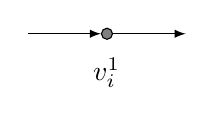
\begin{tikzpicture}
        %nodes
        \node[circle, draw] (a) at (0, 0) {};
        \begin{scope}[every node/.style = {right, anchor = west}]
          \node[xshift=-3mm] at (0, -0.5) {$v_i^1$};
        \end{scope}
        %edges
        \path [draw,-latex] (-1, 0) to (a);
        \path [draw,-latex] (a) to (1, 0);
      \end{tikzpicture}
      \caption{An RCSP example of the VRPTW.}
      \label{fig:vrptw_disposable_example}
    \end{figure}
    \columnbreak  
    \begin{itemize}
      \item \textcolor{blue}{$K = \{1\}$};
      \item \textcolor{blue}{$R^1 = \{f\}$};
      \item \textcolor{blue}{$l_{i,f} = 0 \quad \forall v_i \in V^1$};
      \item \textcolor{blue}{$u_{i,f} = \beta \quad \forall v_i \in V^1$}.
    \end{itemize}
    \begin{figure}[H]
      \centering
      \begin{tikzpicture}
        \tikzstyle{every node}=[circle, draw, fill=black!50, inner sep=0pt, minimum width=4pt]
        %nodes
        \node[triangle] (in) at (-1, 0) {};
        \node[triangle] (out) at (1, 0) {};
        %edges
      \begin{scope}[every node/.style = {right, anchor = west}]
%        \node[xshift=-8mm] at (-1, 1) {$[l_i^k, u_i^k]$};
%        \node[xshift=-6mm] at (-1, 0.5) {$[0, \beta]$};
%        \node[xshift=-8mm] at (1, 1) {$[l_j^k, u_j^k]$};
%        \node[xshift=-6mm] at (1, 0.5) {$[0, \beta]$};
        \node[xshift=-3mm] at (-1, -0.5) {$v_i^1$};
        \node[xshift=-3mm] at (1, -0.5) {$v_j^1$};
        \path [draw,-latex] (in) to node[above]{$-\beta$} (out);
      \end{scope}
        \path [draw,-latex] (-1.5, 0) to (in);
        \path [draw,-latex] (out) to (1.5, 0);
      \end{tikzpicture}
      \caption{An RCSP example of the GVRP.}
      \label{fig:gvrp_disposable_example}
    \end{figure}
    Note that \textcolor{red}{$f \in R^1$} is non-monotone.
  \end{multicols}
\end{frame}

\begin{frame}
  \frametitle{Resource Constrained Shortest Path}
  \framesubtitle{Resources: Main x Secondary}
  \begin{itemize}
    \item \textbf{Main:} 
      \begin{itemize}
        \item Always \textbf{disposable}.
        \item Is directly linked to the definition of the \textbf{bucket graphs} in the \textbf{labeling} algorithm, which improves significantly the \textbf{pricing algorithm} performance when compared with secondary resources;
        \item The first main resource is a special one, since the consumption of the first main resource determines the threshold for the bi-directional labeling algorithm.
      \end{itemize}
    \item \textbf{Secondary:} Can be either monotone or non-monotone, and either disposable or non-disposable
  \end{itemize}
\end{frame}

\begin{frame}
  \frametitle{Resource Constrained Shortest Path}
  \framesubtitle{Resources: Binary x Non-binary}
  A resource \textcolor{blue}{$r \in R^k, \forall k \in K$} is
  \begin{itemize}
    \item \textbf{Binary:} If the conditions below are satisfied 
      \begin{enumerate}
        \item Accumulated consumption \textcolor{blue}{$\in \mathbb{B}$};
        \item \textcolor{blue}{$\forall a \in A^k (d_{a,r} \in \{-1, 0, 1\})$};
        \item \textcolor{blue}{$\forall v \in V^k ((l_{v,r}, u_{v,r}) \in \{(0, 0),  (0, 1), (1, 1)\})$};
        \item Is \textbf{secondary};
        \item If it is \textbf{non-disposable}, then \textcolor{blue}{$l_{v_{\text{sink}}^k,r}, u_{v_{\text{sink}}^k,r} = 0, 1$};
      \end{enumerate}
    \item \textbf{Non-binary:} Otherwise.
  \end{itemize}
  Sets of \textbf{secondary binary resources} of the same type (\textbf{disposable} or \textbf{non-disposable}) are implemented in a special way, being represented as bitsets in the \textbf{labels}. 
  This greatly decreases the time spent for \textbf{dominance checks} between labels.
\end{frame}

\begin{frame}
  \frametitle{Resource Constrained Shortest Path}
  \framesubtitle{Remarks}
  \begin{itemize}
    \item There should not exist a cycle in the subproblem graph \textbf{with zero consumption} of all main resources;
    \item \textbf{Unless} the VrpGraph is \textbf{acyclic}, it is mandatory the existence of at least one main resource;
    \item If the digraph is \textbf{acyclic}, in principle it is possible to \textbf{not have any} resource;
      In this case, an artificial main resource should be defined with zero consumption for all arcs. 
      Also in this case bidirectional labeling should not be used.
  \end{itemize}
\end{frame}

\begin{frame}
  \frametitle{Resource Constrained Shortest Path}
  \framesubtitle{Remarks}
  \begin{itemize}
    \item Note that, some feasible paths \textbf{may not be elementary}, i.e., some vertices or arcs might be visited more than once;
    \item As vertices and arcs in different graphs are distinct, paths in different graphs are also distinct.
    \item Currently, VRPSolver has the following \textbf{limits} for resources in a subproblem digraph:
      \begin{itemize}
        \item at most \textbf{2 main} resources;
        \item at most \textbf{20 non-binary} resources (including main ones);
        \item at most \textbf{512 binary} resources.
      \end{itemize}
  \end{itemize}
\end{frame}
